%! TEX root = /Users/circle/Documents/博二上/湍流/Turbulence/HW4/homework/homework.tex
\documentclass[12pt,a4]{ctexart}
\usepackage{natbib}
\usepackage{url}
\usepackage{stmaryrd}
\usepackage{mathrsfs}
\usepackage{amsmath}
\usepackage{graphicx}
\usepackage{parskip}
\usepackage{fancyhdr}
% \usepackage{underscore} % 下划线
\usepackage{commath}%定义d
\usepackage{geometry}
\usepackage{bm}
\usepackage{siunitx}
\usepackage{float}
% \usepackage[skip=-5pt]{subcaption}
% \usepackage{subfig}
\usepackage{subfigure}  %插入多图时用子图显示的宏包
\usepackage{titlesec}
\usepackage{caption}
\usepackage{paralist}
\usepackage{multirow}
\usepackage{booktabs} % To thicken table lines
\usepackage{diagbox}
\usepackage{authblk}
\usepackage{indentfirst}
\usepackage{amsthm}
\usepackage{fontspec}
\usepackage{color}
%\usepackage{txfonts} %设置字体为times new roman
\usepackage{lettrine}
\usepackage{nameref}
%\usepackage[nottoc]{tocbibind}
\usepackage{amssymb}%font
\usepackage{lipsum}%make test words
\usepackage{picinpar}%words around the picture
\usepackage[all]{xy}%draw arrow
\usepackage{asymptote}%draw picture
\usepackage[perpage]{footmisc}%脚注每页清零
\usepackage{esint}
\renewcommand{\proofname}{\indent \sf \bfseries{证明}}
\pagestyle{fancy}
\fancyhf{}
\renewcommand{\headrulewidth}{0pt}
\fancyfoot[C]{\thepage}

\catcode`\。=\active
\catcode`\,=\active
\catcode`\;=\active
\catcode`\:=\active
\newcommand{。}{.}
\newcommand{,}{,}
\newcommand{;}{;}
\newcommand{:}{:}

\geometry{bottom=3cm,left=3cm,right=3cm,a4paper, top=2.5cm}
% \footskip = 60pt

% \setmainfont{TimesNewRomanPSMT}
% \setsansfont{Helvetica-Light}
\setCJKmainfont[ItalicFont=STKaitiSC-Regular,BoldFont=SimSong-Bold]{SimSong-Regular}
\setCJKsansfont[BoldFont=STHeitiSC-Medium]{STHeitiSC-Light}


%\setmainfont{Times New Roman}

\ctexset{today=old}%日期类型设置

% ======================================
% = Color de la Universidad de Sevilla =
% ======================================
\usepackage{tikz}
\definecolor{PKUred}{cmyk}{0,1,1,0.45}

%超链接设置
\usepackage[breaklinks,colorlinks,linkcolor=PKUred,citecolor=PKUred,pagebackref,urlcolor=PKUred]{hyperref}
\usepackage{cleveref}
\newcommand{\crefpairconjunction}{ 和 }
% \newcommand{\crefmiddleconjunction}{ 和 } 
\newcommand{\creflastconjunction}{ 和 }

\newcommand{\hsp}{\hspace{20pt}}
\newcommand{\nhsp}{\hspace{-30pt}}
% \titleformat{\section}{\Large\bfseries}{%\arabic{section}
% \hspace{-22pt}\textcolor{PKUred}{\vrule width 2pt}\hsp}{0pt}{}


% \titleformat{\subsection}
% {\normalfont\large\bfseries}{}{0em}{}

\renewcommand*\footnoterule{%
   \vspace*{-3pt}%
   {\color{PKUred}\hrule width 2in height 0.4pt}%
   \vspace*{2.6pt}%
}


%% Color the bullets of the itemize environment and make the symbol of the third
%% level a diamond instead of an asterisk.
%h\renewcommand*\textbullet{\dag}
\renewcommand*\labelitemi{\color{PKUred}\textbullet}
\renewcommand*\labelitemii{\color{PKUred}--}
\renewcommand*\labelitemiii{\color{PKUred}$\diamond$}
\renewcommand*\labelitemiv{\color{PKUred}\textperiodcentered}



%%% Equation and float numbering
\numberwithin{equation}{section}		% Equationnumbering: section.eq#
\numberwithin{figure}{section}			% Figurenumbering: section.fig#
\numberwithin{table}{section}				% Tablenumbering: section.tab#


%代码设置
\usepackage{listings}
\usepackage{accsupp}
\usepackage{fontspec} % 定制字体
\newfontfamily\menlo{Menlo-Regular}
\usepackage{xcolor} % 定制颜色
\definecolor{mygreen}{rgb}{0,0.6,0}
\definecolor{mygray}{rgb}{0.5,0.5,0.5}
\definecolor{mymauve}{rgb}{0.58,0,0.82}
\lstset{
   numbers=left,
   numberstyle=\footnotesize\menlo,
   basicstyle=\footnotesize\menlo,
   backgroundcolor=\color{white},      % choose the background color
   columns=fullflexible,
   tabsize=4,
   breaklines=true,               % automatic line breaking only at whitespace
   captionpos=b,                  % sets the caption-position to bottom
   commentstyle=\color{mygreen},  % comment style
   escapeinside={\%*}{*)},        % if you want to add LaTeX within your code
   keywordstyle=\color{blue},     % keyword style
   stringstyle=\color{mymauve}\ttfamily,  % string literal style
   frame=lrtb,
   rulesepcolor=\color{red!20!green!20!blue!20},
   % identifierstyle=\color{red},
   % language=c++,
   xleftmargin=4em,xrightmargin=2em, aboveskip=1em,
   % framexleftmargin=2em,
   numbers=left
}

%脚注
\renewcommand\thefootnote{\fnsymbol{footnote}}

%定义常数i、e、积分符号d
\newcommand\mi{\mathrm{i}}
\newcommand\me{\mathrm{e}}

%%% Maketitle metadata
\newcommand{\horrule}[1]{\rule{\linewidth}{#1}} 	% Horizontal rule
\newcommand{\tabincell}[2]{\begin{tabular}{@{}#1@{}}#2\end{tabular}}


\setcounter{secnumdepth}{2}
\usepackage{bm}
\usepackage{autobreak}
\usepackage{amsmath}
\setlength{\parindent}{2em}
\graphicspath{{../code/}}


%pdf 文件设置
\hypersetup{
   pdfauthor={袁磊祺},
   pdftitle={湍流4}
}

\title{
   \vspace{-1in}
   \usefont{OT1}{bch}{b}{n}
   \normalfont \normalsize \textsc{\LARGE Peking University}\\[1cm] % Name of your university/college \\ [25pt]
   \horrule{0.5pt} \\[0.5cm]
   \huge \bfseries{湍流4} \\
   \horrule{2pt} \\[0.5cm]
}
\author{
   \normalfont									\normalsize
   College of Engineering \quad 2001111690  \quad 袁磊祺\\	\normalsize
   \today
}
\date{}

\begin{document}

%%%%%%%%%%%%%%%%%%%%%%%%%%%%%%%%%%%%%%%%%%%%%%
\captionsetup[figure]{name={图},labelsep=period}
\captionsetup[table]{name={表},labelsep=period}
\renewcommand\contentsname{目录}
\renewcommand\listfigurename{插图目录}
\renewcommand\listtablename{表格目录}
\renewcommand\refname{参考文献}
\renewcommand\indexname{索引}
\renewcommand\figurename{图}
\renewcommand\tablename{表}
\renewcommand\abstractname{摘\quad 要}
\renewcommand\partname{部分}
\renewcommand\appendixname{附录}
\def\equationautorefname{式}%
\def\footnoteautorefname{脚注}%
\def\itemautorefname{项}%
\def\figureautorefname{图}%
\def\tableautorefname{表}%
\def\partautorefname{篇}%
\def\appendixautorefname{附录}%
\def\chapterautorefname{章}%
\def\sectionautorefname{节}%
\def\subsectionautorefname{小小节}%
\def\subsubsectionautorefname{subsubsection}%
\def\paragraphautorefname{段落}%
\def\subparagraphautorefname{子段落}%
\def\FancyVerbLineautorefname{行}%
\def\theoremautorefname{定理}%
\crefname{figure}{图}{图}
\crefname{equation}{式}{式}
\crefname{table}{表}{表}
%%%%%%%%%%%%%%%%%%%%%%%%%%%%%%%%%%%%%%%%%%%

\maketitle

2021 年 1 月 3 日前交电子版.

代码等作业内容可在 \texttt{\href{https://github.com/circlelq/Turbulence}{https://github.com/circlelq/Turbulence}} 查看。


\section{1}

自己构造一个在适当的小尺度范围满足 “ $2 / 3$ ” 定律的二阶纵向速度结构函数, 画出结构函数和一维能谱, 考察能谱函数是否满足 “ $5 / 3$ ” 定律。

\textsf{\hspace{-2em}\sf  \textbf{解:}}

已知$B_{d d}$ 和$E(k)$的表达式为\cite{shi}
\begin{equation}
   B_{d d} = 2 \overline{u^2} [1 - E(r)],
\end{equation}
\begin{equation}
   E(k) = \frac{1}{\pi} \int_{0}^{+\infty} \overline{u^2}f(r)(kr)^2\left( \frac{\sin kr}{kr} - \cos kr \right) \dif r.
   \label{eq:1-1}
\end{equation}
下面构造$B_{d d}$,由于$f(0)=0$, $\lim_{r \to +\infty} f(r) = 0$, 所以设
\begin{equation}
   B_{d d}(r) = \begin{cases}
	  r^{\frac{2}{3}} , & r < 0.9, \\
	  1 - \left(\frac{1 - 0.9^{\frac{2}{3}}}{1 - \tanh(0.9)}\right)(1 - \tanh(r)), & r \ge  0.9.
   \end{cases}
\end{equation}

假设所有系数都为$1$,则可以画图像得\cref{fig:1-1}.
画能谱可得\cref{fig:1-2},可见能谱不一定满足$5 / 3$ 定律,因为\cref{eq:1-1}的积分式子很容易让函数发散,很难让$E$ 渐进趋于$0$.
\begin{figure}[htpb]
   \centering
   \subfigure[二阶纵向速度结构函数$B_{d d}$.]{\label{fig:1-1}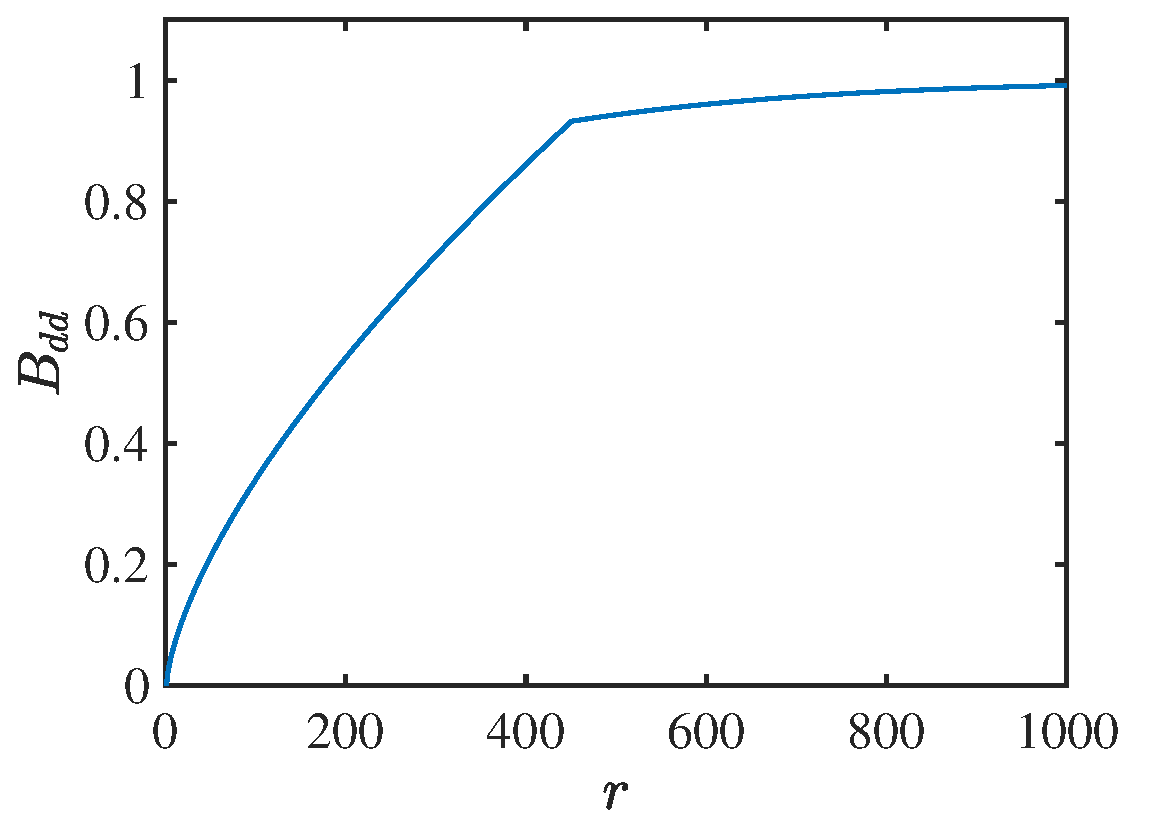
\includegraphics[width=.45\textwidth]{question1-1.eps}}\quad
   \subfigure[能谱.]{\label{fig:1-2}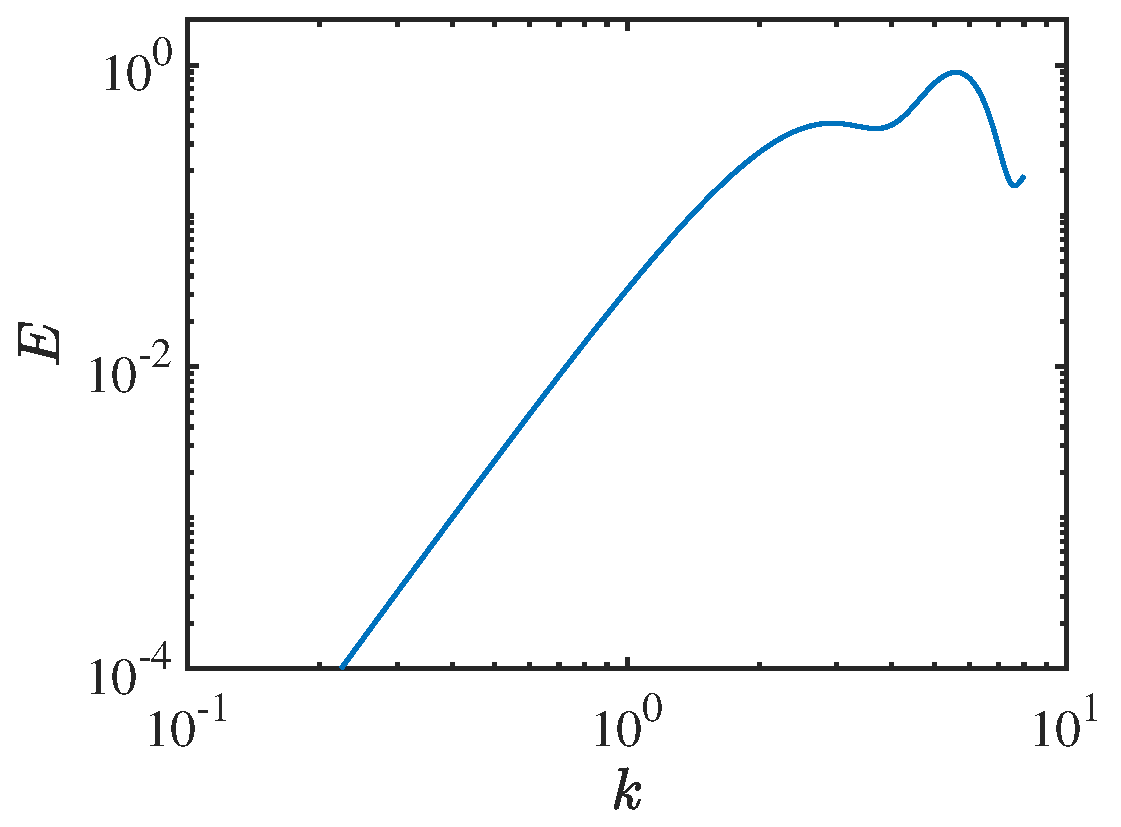
\includegraphics[width=.45\textwidth]{question1-2.eps}}\quad
   \caption{二阶纵向速度结构函数$B_{d d}$和能谱.}
\end{figure}



\section{2}

考虑均匀各向同性湍流早期的衰减过程, 用 Pao (鲍亦和) 的能量传递模型和 相似性解数值求解无量纲的三维能谱函数, 并在一张图上画出若干初始雷诺数 下的无量纲能谱函数曲线。

\textsf{\hspace{-2em}\sf  \textbf{解:}}

卡门--豪沃思方程的积分形式为
\begin{equation}
   \frac{\partial }{\partial t}  \int_{0}^{k} E(k',t)\dif k' = -S(k,t) - 2\nu \int_{0}^{k} k'^2E(k',t)\dif k'.  
   \label{eq:2_1}
\end{equation}

Pao YH 模型 \cite{PaoYH}
\begin{equation}
   S=\sigma(k) E(k)=\alpha^{-1} \varepsilon^{\frac{1}{3}} k^{\frac{5}{3}} E(k).
\end{equation}

原文献和书上(\cite{shi})写的并不一样,根据 \cite{10.2307/98337} 的假设有
\begin{equation}
   \frac{\partial}{\partial t} \int_{0}^{k} E(k', t) \dif  k'=-\left\{\nu+\kappa \int_{k}^{\infty} \sqrt{\left(\frac{E^{\prime}\left(k^{'}, t\right)}{k^{' 3}}\right)} \dif  k^{'}\right\} \int_{0}^{k} 2 E^{\prime}\left(k^{\prime}, t\right) k^{\prime 2} \dif k^{\prime} .
\end{equation}
假设
\begin{equation}
   E(k,t) = \frac{1}{\sqrt{t} } f(k\sqrt{t}),
   \label{eq:2_2}
\end{equation}
可得
\begin{equation}
   \int_{0}^{x} f(x') \dif x'-\frac{1}{2} x f(x)=\left\{\nu+\kappa \int_{x}^{\infty} \sqrt{\frac{f\left(x^{'}\right)}{x^{' 3}}}  \dif x^{'}\right\} \int_{0}^{x} 2 f\left(x^{\prime}\right) x^{\prime 2} \dif x^{\prime}.
\end{equation}

若将Pao YH模型代入\cref{eq:2_1},并利用同样的相似性假设\cref{eq:2_2},得到的方程并不能将时间$t$ 约掉,可能需要别的相似性假设才能得到可以求解的方程。



\section{3}

阅读 Kolmogorov 1941 年的三篇湍流经典论文 \citep{kolmogorov1941dit} (见分享的书 Turbulence: Classical papers on statistical theory) 。 对较少关注的第二篇论文, 在你阅读后用 最简洁的论证给出 “$-10/7$” 衰减规律。并问用类似的方法, 通过适当修改假设, 可否推出湍流动能的指数规律衰减规律 (有人在一定形状的分形格栅尾流中测 量到此规律)?

\textsf{\hspace{-2em}\sf  \textbf{解:}}

对于各向同性湍流,假设单位质量的平均能量是$3/2 b$,则单位时间单位质量的能量耗散是
\begin{equation}
   \overline{\varepsilon} = - \frac{3}{2} \frac{\dif b}{\dif t}.
   \label{eq:3-1}
\end{equation}
由假设有
\begin{equation}
   \overline{\varepsilon} = \left( \frac{2gb}{C} \right) ^{\frac{3}{2}} L^{-1},
\end{equation}
\begin{equation}
   L = \left( \frac{\Lambda}{b} \right)^{\frac{1}{5}},
\end{equation}
\begin{equation}
   K = \frac{2}{3} \left( \frac{2g}{C} \right)^{\frac{3}{2}},
\end{equation}
其中$K$是常数,所以
\begin{equation}
   \frac{\dif b}{\dif t} = - K \Lambda^{-\frac{1}{5}} b^{\frac{17}{10}}.
\end{equation}
积分可得
\begin{equation}
   b = \left( \frac{10}{rK} \right)^{\frac{10}{7}} \Lambda^{\frac{2}{7}} (t-t_0)^{-\frac{10}{7}}.
\end{equation}
代入\cref{eq:3-1}有
\begin{equation}
   \overline{\varepsilon} = \frac{15}{7} \left( \frac{10}{rK} \right)^{\frac{10}{7}} \Lambda^{\frac{2}{7}} (t-t_0)^{-\frac{17}{7}} .
\end{equation}






\section{4}

证明 She--Leveque 层次相似律(Hierarchical Self--Similarity, HSS)是广义扩展自 相似律(Generalized Extended Self--Similarity, GESS)的一个特殊情形。

\cite{Emily02} 这篇文章讨论了这个问题。

Fully developed turbulence is characterized by powerlaw dependence of the moments of velocity fluctuations. It was suggested by Kolmogorov in 1941 (K41) that there is a constant rate of energy transfer from large to small scales and that the statistical properties of the velocity difference across a separation $r, \delta v_{r} \equiv v(x+r)-v(x)$, depend only on the mean energy transfer or equivalently the mean energy dissipation rate $\epsilon$ and the scale $r$ when $r$ is within an inertial range. Dimensional considerations then lead to the prediction that the velocity structure functions, which are moments of the magnitude of the velocity difference, have simple power-law dependence on $r$ within the inertial range:
\begin{equation}
   S_{p}(r) \equiv\left\langle\left|\delta v_{r}\right|^{p}\right\rangle \sim \epsilon^{p / 3} r^{p / 3}
\end{equation}
Experiments have indicated that there is indeed power law scaling in the inertial range but the scaling exponents are different from $p / 3$ :
\begin{equation}
   S_{p}(r) \sim r^{\zeta_{p}}
\end{equation}
where $\zeta_{p}$ has a nonlinear dependence on $p$. Such a deviation implies that the functional form of the probability density function (pdf) of $\delta v_{r}$ depends on $r$, that is, the velocity fluctuations have scale-dependent statistics. Understanding this deviation from K41 is essential to our fundamental understanding of the small scale statistical properties of turbulence.

A number of phenomenological models have been proposed to explain the anomalous scaling exponents $\zeta_{p}$. Among them, a recent successful one is from She and Leveque with a hypothesis of a hierarchical structure (HS). When stated for the velocity structure functions, the HS hypothesis reads
\begin{equation}
   \frac{S_{p+2}(r)}{S_{p+1}(r)}=A_{p+1}\left[\frac{S_{p+1}(r)}{S_{p}(r)}\right]^{\beta}\left[S^{(\infty)}(r)\right]^{1-\beta},
   \label{eq:4-1}
\end{equation}

Here $S^{(\infty)}(r) \equiv \lim _{p \rightarrow \infty} S_{p+1}(r) / S_{p}(r)$ and $0<\beta<1$ is a constant. This hypothesis (and the similar version for the local energy dissipation) was supported by experimental velocity measurements taken in turbulent jets and wakes. Note that the boundedness of the velocity will ensure the existence of $S^{(\infty)}(r)$. In fact, one can show that $S^{(\infty)}(r) \equiv \lim _{p \rightarrow \infty} S_{p}^{1 / p}$, and is equal to $\left|\delta v_{r}\right|^{\max }$, the maximum magnitude of $\delta v_{r}$.

In this Letter, we shall show that the She--Leveque hierarchical structure (SLHS) leads to GESS. In other words, the SLHS is a special form of GESS. We then give a generalized form of SLHS, which is equivalent to GESS, with the constant $\beta$ replaced by a function of $p$.

First, rewrite Eq. (\ref{eq:4-1}) as
\begin{equation}
   \frac{S_{k+1}(r)}{S_{k}(r) S^{(\infty)}(r)}=A_{k}\left[\frac{S_{k}(r)}{S_{k-1}(r) S^{(\infty)}(r)}\right]^{\beta}
\end{equation}
for integer $k$, which implies
\begin{equation}
   \frac{S_{k}(r)}{S_{k-1}(r) S^{(\infty)}(r)}=\Pi_{j=0}^{k-1} A_{j}^{\beta^{k-1-j}}\left[\frac{S_{1}(r)}{S^{(\infty)}(r)}\right]^{\beta^{k-1}}
   \label{eq:4-2}
\end{equation}
ultiply Eq. (\ref{eq:4-2}) for $k=1,2, \ldots, n$ gives
\begin{equation}
   S_{n}(r)=B_{n}\left[\frac{S_{1}(r)}{S^{(\infty)}(r)}\right]^{\frac{1-\beta^{n}}{1-\beta}}\left[S^{(\infty)}(r)\right]^{n}
\end{equation}
where $B_{n} \equiv \Pi_{k=1}^{n} \Pi_{j=0}^{k-1} A_{j}^{\beta^{k-1-j}}$, which further gives
\begin{equation}
   \frac{S_{n}(r)}{S_{3}(r)^{n / 3}}=\frac{B_{n}}{B_{3}^{n / 3}}\left[\frac{S_{1}(r)}{S^{(\infty)}(r)}\right]^{\frac{3\left(1-\beta^{n}\right)-n\left(1-\beta^{3}\right)}{3(1-\beta)}}
   \label{eq:4-3}
\end{equation}
Equation (\ref{eq:4-3}) then implies the GESS property:
\begin{equation}
   T_{n}(r) \sim T_{m}(r)^{\rho(n, m)}
\end{equation}
which is a scaling behavior for the normalized structure functions, $T_{n}(r) \equiv S_{n}(r) / S_{3}(r)^{n / 3}$, with the normalized exponents $\rho(n, m)$ even when $S_{n}(r)$ does not have a scaling behavior in $r$. For SLHS,
\begin{equation}
   \rho(n, m)=\frac{3\left(1-\beta^{n}\right)-n\left(1-\beta^{3}\right)}{3\left(1-\beta^{m}\right)-m\left(1-\beta^{3}\right)}
\end{equation}
We have thus proved that SLHS implies GESS.\qed



\section{5}

K62 \citep{kolmogorov_1962} 模型中假设湍流在尺度 $\ell$ 上的粗粒化耗散率 $\varepsilon_{\ell}$ 满足对数正态分布, 并且均值和方差也满足随尺度变化的一定的对数规律, 由此推出 $p$ 阶速度结构函数的标度指数规律为 $\zeta(p)=\frac{p}{3}+\frac{\mu p}{18}(3-p)$ 。

证明: 尺度 $\ell$ 上速度增量的绝对值 $U$ 作为随机变量, 其概率密度 $P(\ell, U)$ 也符合对数正态分布, 且满足如下方程:
\begin{equation}
   \ell \frac{\partial P}{\partial \ell}+(\gamma+4 b) U \frac{\partial P}{\partial U}+b U^{2} \frac{\partial^{2} P}{\partial U^{2}}+(\gamma+2 b) P=0,
   \label{eq:5-1}
\end{equation}
其中 $\gamma=(3+\mu) / 9, b=\mu / 18$ 。

根据\cite[P71]{zhang17}有,用量纲分析导出改进的Kolmogorov模型是
\begin{equation}
   \delta u_l \propto (\varepsilon_{\ell} r)^{\frac{1}{3}}, 
\end{equation}
设比例系数是$b$,两边取对数得
\begin{equation}
   \ln \delta u_{\ell} = \ln b + \frac{1}{3} \ln \ell + \frac{1}{3} \ln \varepsilon_{\ell}, 
\end{equation}
由于$\ln \varepsilon_{\ell}$ 是正态分布,所以$\delta u$ 是对数正态分布。由根据对数假设有
\begin{equation}
   p(\varepsilon_{\ell}) = \frac{1}{\sqrt{2\pi} \sigma} \frac{1}{\varepsilon_{\ell}} \me^{-\frac{\left( \ln \varepsilon_{\ell} - a \right)^2 }{2 \sigma^2}},
\end{equation}
\begin{equation}
   \left< \left( \ln \varepsilon_{\ell} - a \right)^2  \right> = \sigma(r) = \mu \ln \frac{r_0}{r} + A,
\end{equation}
\begin{equation}
   a(r) = c\ln \frac{r_0}{r} + a_0.
\end{equation}
由此可得\cref{eq:5-1}.\qed


\section{6}

试估计用大涡模拟方法计算高雷诺数边界层湍流时的网格规模。参考 Pope 书
习题 13.29 (A) 推出 (13.173) 式。


\textsf{\hspace{-2em}\sf  \textbf{解:}}

In LES-NWR, in order to resolve the near-wall motions, the filter width and grid spacing in the viscous near-wall region must be on the order of $\delta_{\nu}$.\cite{pop} So 
\begin{equation}
   \Delta x=a_{x} \delta_{v}, \quad \Delta z=a_{z} \delta_{v}.
\end{equation}
where $a_x$ and $a_z$ are positive constants.\qed



\section{7}

Prandtl 混合长模型是应用最多的一个湍流模型。但教科书中通常都是针对平
均流动为二维单向的剪切湍流给出给模型。试给出混合长模型的一个三维各向
异性推广。注意: 模型应符合坐标不变的张量性质。


\textsf{\hspace{-2em}\sf  \textbf{解:}}

下文对Prandtl混合长模型的描述来自\cite{pop}.

The turbulent viscosity $\nu_{\mathrm{T}}(y)$ is defined so that the Reynolds shear stress is given by
\begin{equation}
   -\langle u v\rangle= \nu_{\mathrm{T}} \frac{\mathrm{d}\langle U\rangle}{\mathrm{d} y} .
   \label{eq:7-1}
\end{equation}
It can be expressed as the product of a velocity scale $u^{*}$ and a lengthscale $\ell_{\mathrm{m}}$ :
\begin{equation}
   \nu_{\mathrm{T}}=u^{*} \ell_{\mathrm{m}} .
   \label{eq:7-2}
\end{equation}
One of these scales can be specified at will, and then the other determines $\nu_{\mathrm{T}}$. A propitious (implicit) specification is
\begin{equation}
   u^{*}=|\langle u v\rangle|^{1 / 2} .
   \label{eq:7-3}
\end{equation}
By substituting Eqs. (\ref{eq:7-2}) and (\ref{eq:7-3}) into Eq. (\ref{eq:7-1}) and taking the absolute value we obtain the explicit relation
\begin{equation}
   u^{*}=\ell_{\mathrm{m}}\left|\frac{\mathrm{d}\langle U\rangle}{\mathrm{d} y}\right| .
   \label{eq:7-4}
\end{equation}
(In the upper half of the channel $(\delta<y<2 \delta)$ the velocity gradient $\mathrm{d}\langle U\rangle / \mathrm{d} y$ is negative and the Reynolds stress $\langle u v\rangle$ is positive. The absolute values in Eqs. (\ref{eq:7-3}) and (\ref{eq:7-4}) ensure that $u^{*}$ is non-negative for all $y$.)

In the overlap region $\left(50 \delta_{v}<y<0.1 \delta\right)$ that occurs at high Reynolds number, the shear stress $-\langle u v\rangle$ differs little from $u_{\tau}^{2}$, and the mean velocity gradient is $u_{\tau} /(\kappa y)$. Consequently, $u^{*}$ equals $u_{\tau}$, and then Eq. (\ref{eq:7-4}) determines $\ell_{m}$ to be
\begin{equation}
   \ell_{\mathrm{m}}=\kappa y .
\end{equation}
Like $L \equiv k^{3 / 2} / \varepsilon$, the lengthscale $\ell_{m}$ varies linearly with $y .$
The above relations constitute Prandtl's mixing-length hypothesis (Prandtl 1925). In summary, the turbulent viscosity is given by
\begin{equation}
   \nu_{\mathrm{T}}=u^{*} \ell_{\mathrm{m}}=\ell_{\mathrm{m}}^{2}\left|\frac{\mathrm{d}\langle U\rangle}{\mathrm{d} y}\right|.
\end{equation}


\subsection{The mixing-length model}

In application to two-dimensional boundary-layer flows, the mixing length $\ell_{\mathrm{m}}(x, y)$ is specified as a function of position, and then the turbulent viscosity is obtained as
\begin{equation}
   \nu_{\mathrm{T}}=\ell_{\mathrm{m}}^{2}\left|\frac{\partial\langle U\rangle}{\partial y}\right|
   \label{eq:7-5}
\end{equation}
As shown in Section 7.1.7, in the log-law region, the appropriate specification of the mixing length is $\ell_{\mathrm{m}}=\kappa y$, and then the turbulent viscosity is $\nu_{\mathrm{T}}=u_{\tau} \kappa y$.
Several generalizations of Eq. (\ref{eq:7-5}) have been proposed in order to allow the application of the mixing-length hypothesis to all flows. On the basis of the mean rate of strain $\bar{S}_{i j}$ Smagorinsky (1963) proposed
\begin{equation}
   \nu_{\mathrm{T}}=\ell_{\mathrm{m}}^{2}\left(2 \bar{S}_{i j} \bar{S}_{i j}\right)^{1 / 2}=\ell_{\mathrm{m}}^{2} \mathcal{S},
\end{equation}
whereas, on the basis of the mean rate of rotation $\bar{\Omega}_{i j}$, Baldwin and Lomax (1978) proposed
\begin{equation}
   \nu_{\mathrm{T}}=\ell_{\mathrm{m}}^{2}\left(2 \bar{\Omega}_{i j} \bar{\Omega}_{i j}\right)^{1 / 2}=\ell_{\mathrm{m}}^{2} \Omega
\end{equation}
(Both of these formulae reduce to Eq. (\ref{eq:7-5}) in the case that $\partial\left\langle U_{1}\right\rangle / \partial x_{2}$ is the only non-zero mean velocity gradient.)


\section{8}

推导周期边界条件下 Navier--Stokes 方程在傅立叶谱空间中的形式。从数学形 式上看, 二维和三维情况下最后有区别吗? 用周期边界条件模拟高雷诺数均匀 各向同性湍流, 在模拟时计算参数的选取应注意什么问题?


\textsf{\hspace{-2em}\sf  \textbf{解:}}

三维 $\bm{u} (\bm{x} ,t)$ , 周期边界条件。\citep[P211]{pop}

\begin{equation}
   \bm{u} (\bm{x} , t) = \sum_{\bm{k} }^{} \hat{\bm{u} } (\bm{k} ,t) \me^{\mi \bm{k} \cdot \bm{x} },
\end{equation}
\begin{equation}
   \nabla \cdot \bm{u} = 0 \implies \sum_{k}^{} \mi \bm{k} \cdot \hat{\bm{u} } (\bm{k} ,t) \me^{\mi \bm{k} \cdot \bm{x} } = 0 \implies \bm{k} \cdot \hat{\bm{u} }(\bm{k} ,t)=0, 
\end{equation}
\begin{equation}
   \frac{\partial \bm{u} }{\partial t}  + \nabla \cdot (\bm{u} \bm{u} ) = - \nabla \left( \frac{p}{\rho} \right) + \nu \nabla ^2 \bm{u} + \bm{f}.
\end{equation}
亥姆霍兹分解 $\bm{a} = \nabla \phi + \bm{a}_{\bot}$
\begin{equation}
   -k^2 \hat{\phi} = \mi \bm{k}  \cdot \hat{\bm{a} }(\bm{k} ),\quad \hat{\phi} = - \frac{\mi \bm{k} }{k^2} \cdot \hat{\bm{a} }(\bm{k} )
\end{euation}
\begin{equation}
   \hat{\bm{a} }_{\bot} = \hat{\bm{a} } - \mi \bm{k} \hat{\phi} = \hat{\bm{a} } + \mi \bm{k} \frac{\mi \bm{k} }{k^2}\cdot \hat{\bm{a} } = \hat{\bm{a} } - \frac{\bm{k} \bm{k} }{k^2}\cdot \hat{\bm{a} } = \left( I - \frac{\bm{k} \bm{k} }{k^2} \right) \cdot \hat{\bm{a} } = P \cdot \hat{\bm{a} }
\end{equation}
其中
\begin{equation}
   P_{ij} = \delta_{ij} - \frac{k_i k_j}{k^2}
\end{equation}
ODE:
\begin{equation}
   \left( \frac{\dif }{\dif t} + \nu k^2 \right) \hat{u}_i (\bm{k} ,t) = - \mi k_m P_{ij} (\bm{k} )  \sum_{\bm{p} + \bm{q} = \bm{k} }^{} u_j (\bm{p} ,t) u_m(\bm{q} ,t) + \hat{f}_i(\bm{k} ,t)
\end{equation}

\begin{equation}
   \sum_{k-\frac{1}{2}\le \abs{\bm{k} }\le k + \frac{1}{2}}^{} \left< \abs{ \hat{u}_i \hat{u}_i } \right> = E(k)
\end{equation}


从数学形式上看,二维和三维情况下最后没有区别。

模拟的时候要注意网格数量和计算的最大波数$k$,使得能解析Kolmogorov 尺度 $\frac{L}{N} \sim \eta$ 
\begin{equation}
   \eta \equiv \left( \frac{\nu^{3}}{\varepsilon} \right)^{\frac{1}{4}}.
\end{equation}







% \nocite{*}

% \newpage
\bibliographystyle{plain}
% \clearpage
\phantomsection

\addcontentsline{toc}{section}{参考文献} %向目录中添加条目,以章的名义
\bibliography{homework}

\end{document}
